\documentclass{article}
\usepackage[left=2cm,right=2cm,top=3cm,bottom=3cm,letterpaper]{geometry}
\usepackage[spanish]{babel}
\usepackage[utf8]{inputenc}
\usepackage{graphicx}
\usepackage{enumitem}
\usepackage{hyperref}

\title{Manual	 de	 introducción,	 instalación	 y	 uso	 de	 Github	 en	 forma	 colaborativa}
\author{Juan Carlos López López \and Adolfo Marín Arriaga \and Luis Rodrigo Rojo Morales}
\date{\today\\}

\begin{document}
 \maketitle



 \begin{itemize}

   \item Introducción:

    Github es una plataforma la cual nos permite hacer desarrollo colaborativo de una manera mas sencilla, utiliza el control de versiones Git. Es de gran ayuda para llevar un orden de que es lo que realiza cada persona, poder regresar a un estado previo del proyecto, tener varias ramas de desarrollo, entre otros.
   \item Instalación:
    \begin{enumerate}
      \item Crear una cuenta en github: https://github.com/


      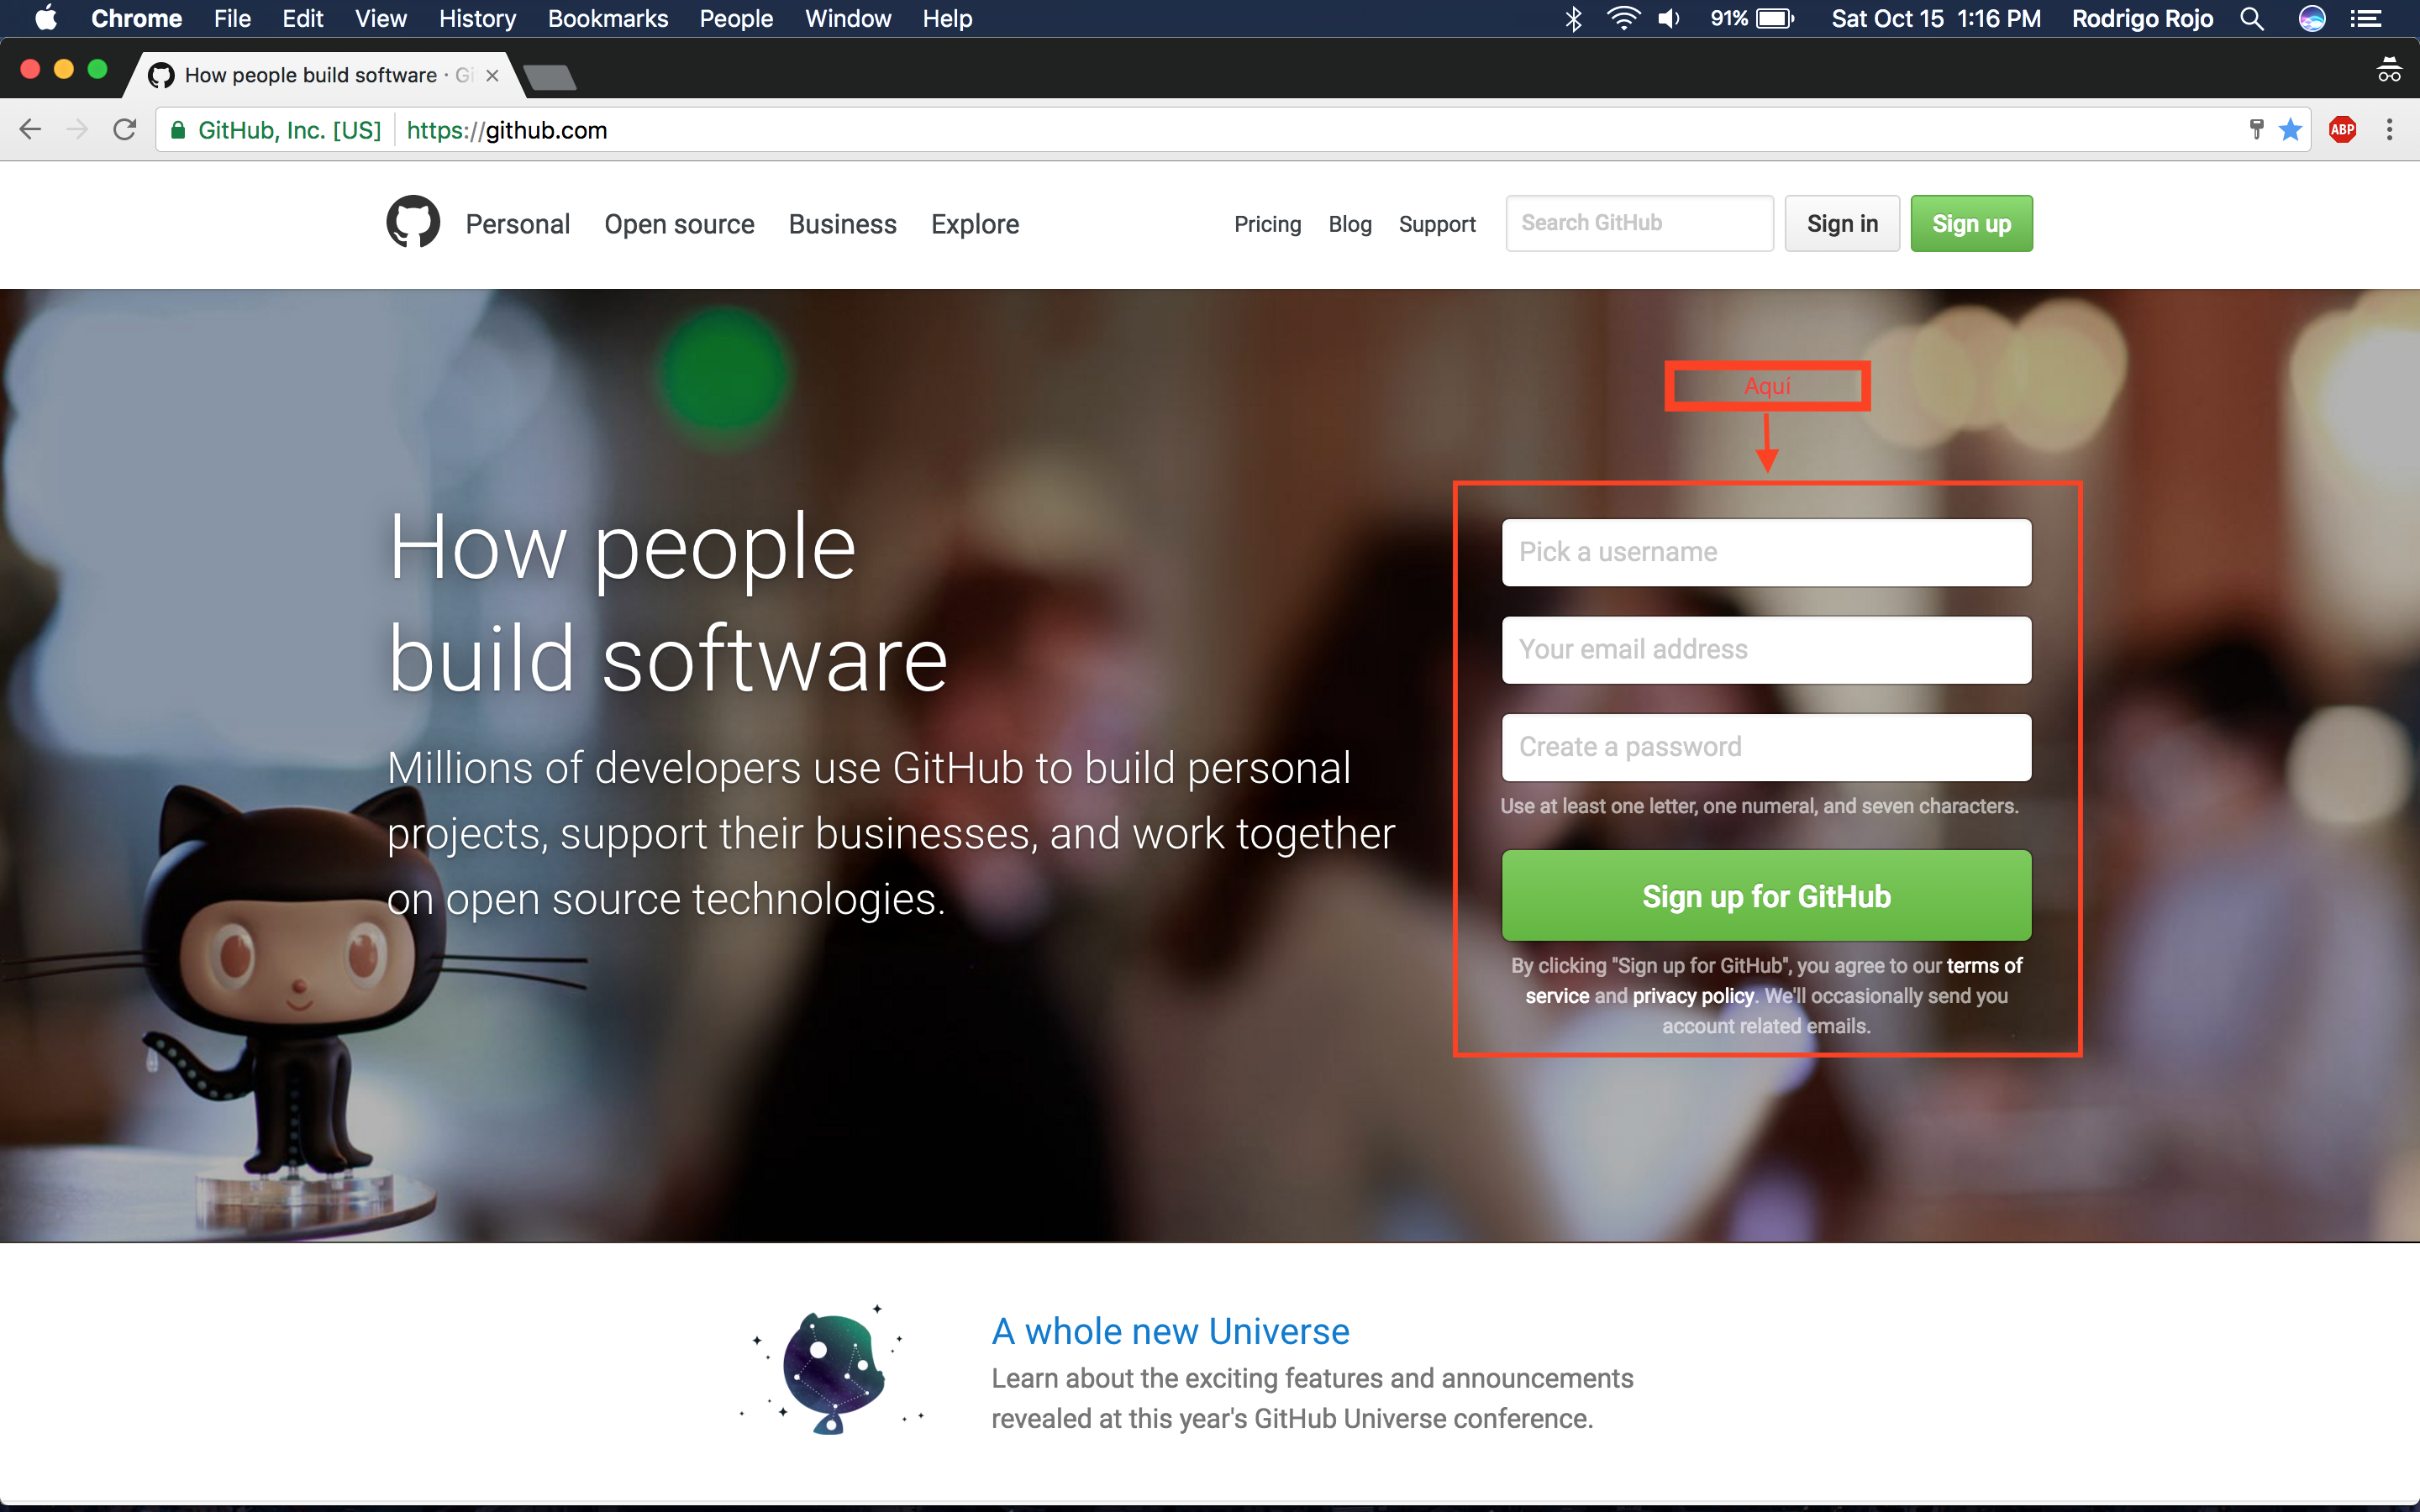
\includegraphics[scale=0.3]{1}

      \item Instalar git:

      Sistema Operativo Ubuntu:
      \begin{verbatim}
        $ sudo apt-get install git
      \end{verbatim}
      Sistema Operativo MacOS:
      \begin{verbatim}
        $ brew install git
      \end{verbatim}

      \item{Configuramos nuestro nombre y correo:}
      \begin{verbatim}
        $ git config --global user.name "YOUR NAME"

        $ git config --global user.email "YOUR EMAIL ADDRESS"
      \end{verbatim}

      \item Creamos una llave SSH y la agregamos al ssh-agent:
      \begin{verbatim}
        $ ssh-keygen -t rsa -b 4096 -C "your_email@example.com"
      \end{verbatim}
      Después de ingresar esto pedirá que ingreses un archivo donde guardar la llave, solo dar enter.
      \begin{verbatim}
        Enter a file in which to save the key (/Users/you/.ssh/id_rsa): [Press enter]
      \end{verbatim}
      Ahora pedirá ingresar frase de seguridad:
      \begin{verbatim}
        Enter passphrase (empty for no passphrase): [Type a passphrase]
        Enter same passphrase again: [Type passphrase again]
      \end{verbatim}
      Para agregar la llave al ssh-agent, primero nos aseguramos que este habilitado:
      \begin{verbatim}
        $ eval "$(ssh-agent -s)"
        Agent pid 59566
      \end{verbatim}
      Agregamos la llave al ssh-agent:
      \begin{verbatim}
        $ ssh-add ~/.ssh/id_rsa
      \end{verbatim}

      \item Agregamos la nueva llave a nuestra cuenta de Github:

      Abrimos una terminal e ingresamos lo siguiente:
      \begin{verbatim}
        $ pbcopy < ~/.ssh/id_rsa.pub
      \end{verbatim}
      Esto nos sirve para copiar la llave al clipboard.\\

      En la parte derecha de cualquier página en Github aparecerá nuestra foto de perfil, le damos click, después sale un menú, le damos click en \textit{Settings}:
      \begin{center}
        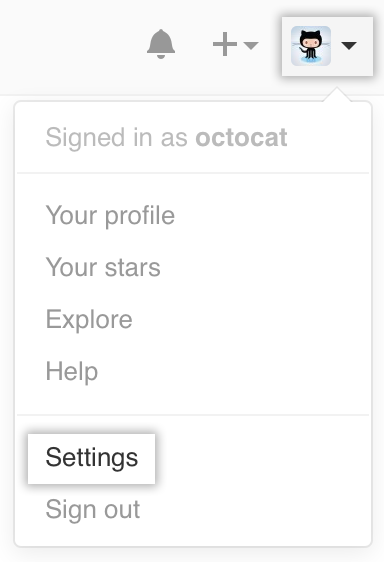
\includegraphics[scale=0.3]{2}
      \end{center}

      Del lado izquierdo nos aparecerá un menú, seleccionamos \textit{SSH and GPG Key}:
      \begin{center}
        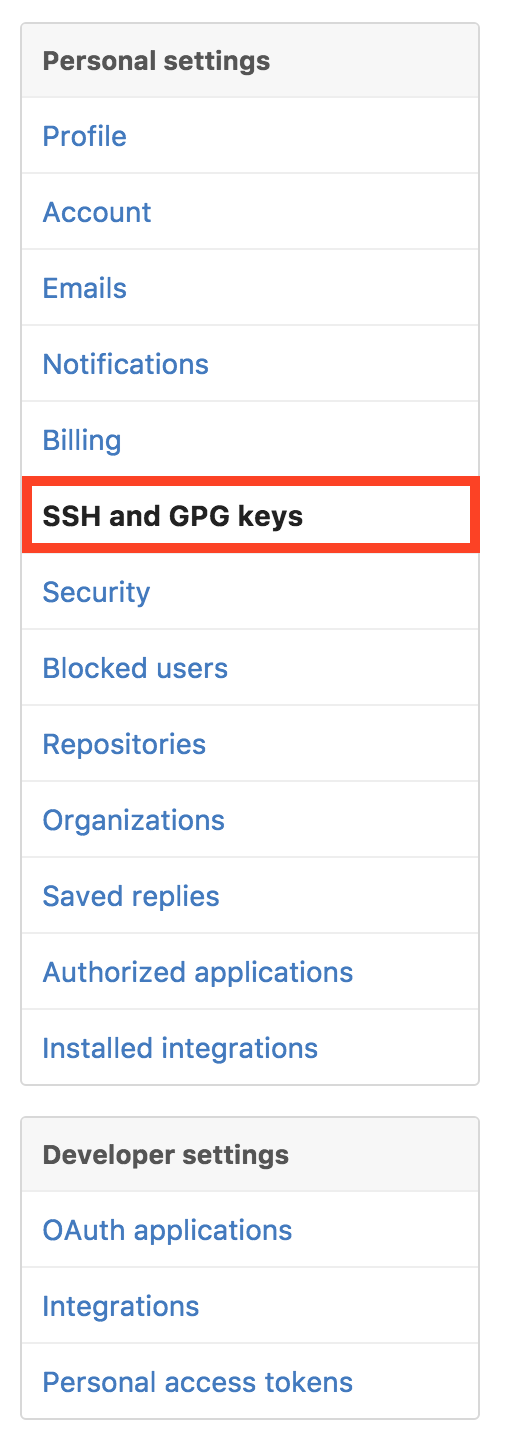
\includegraphics[scale=0.3]{3}
      \end{center}

      Le damos click en el boton de \textit{New Key}:
      \begin{center}
        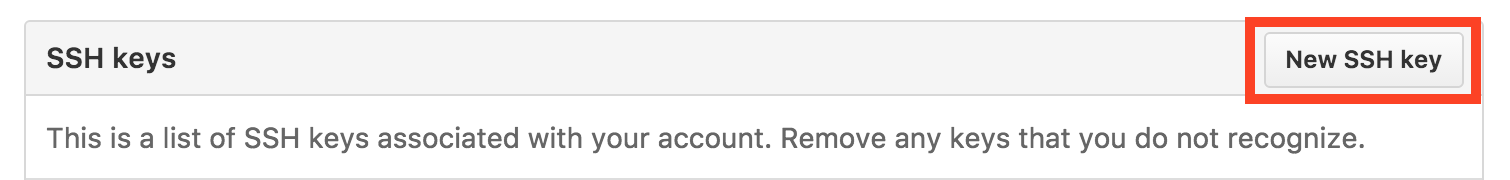
\includegraphics[scale=0.3]{4}
      \end{center}

      Llenamos los datos correspondientes, en \textit{Title} le ponemos con el que la vayamos a identificar, y en \textit{Key} hacemos ctrl+v porque previamente ya la habíamos copiado.
      \begin{center}
        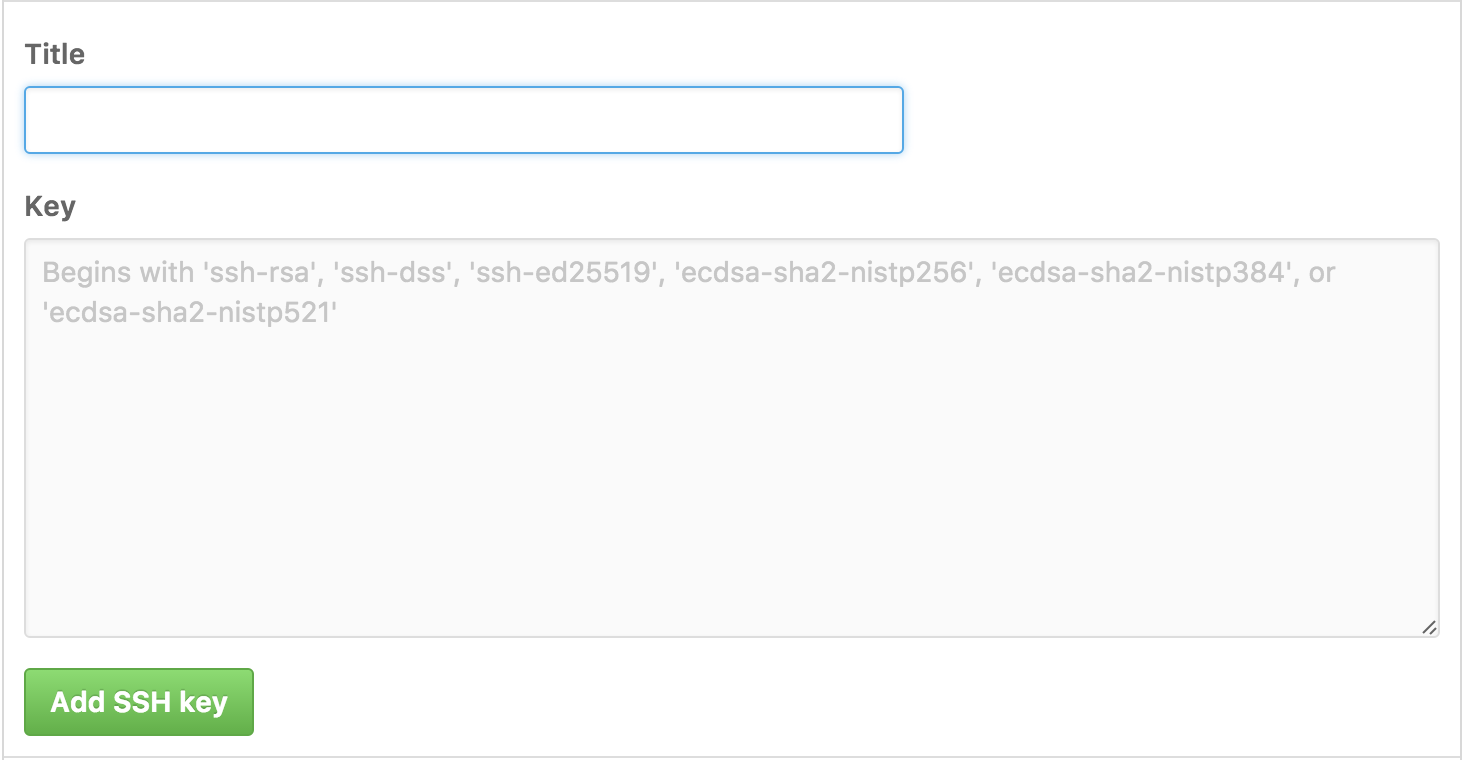
\includegraphics[scale=0.4]{5}
      \end{center}

      Posteriormente le damos click en el botón verde \textit{Add SSH Key} y nos pedirá que ingresemos nuestra contraseña.

    \end{enumerate}

   \item Uso:
   \begin{enumerate}
     \item Una vez realizados los pasos previamente ya podemos hacer uso de git y Github. Ahora tendremos que crear un repositorio, esto lo haremos desde https://github.com/new, ingresamos los datos, en este caso los del Proyecto Final:
     \begin{center}
       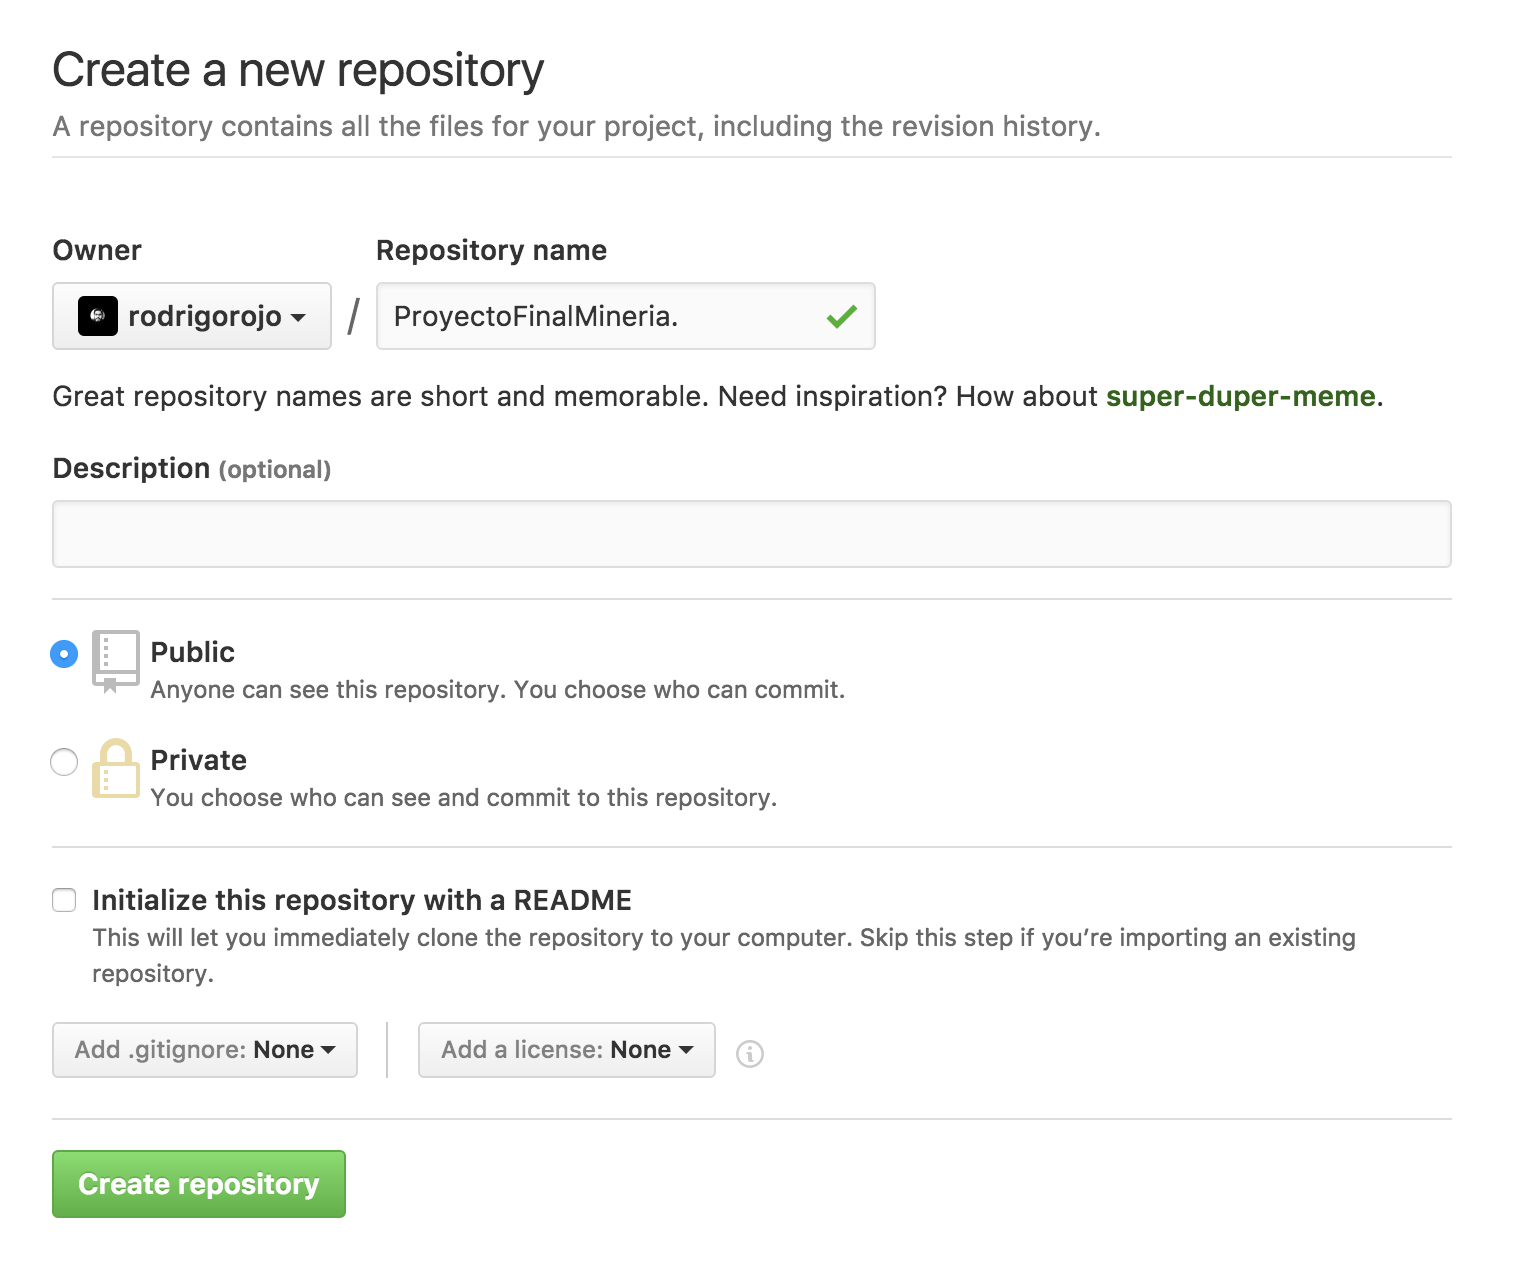
\includegraphics[scale=0.5]{6}
     \end{center}
     y le damos click en \textit{Create repository}
     \item Ahora agregamos a los colaboradores:
     \begin{center}
       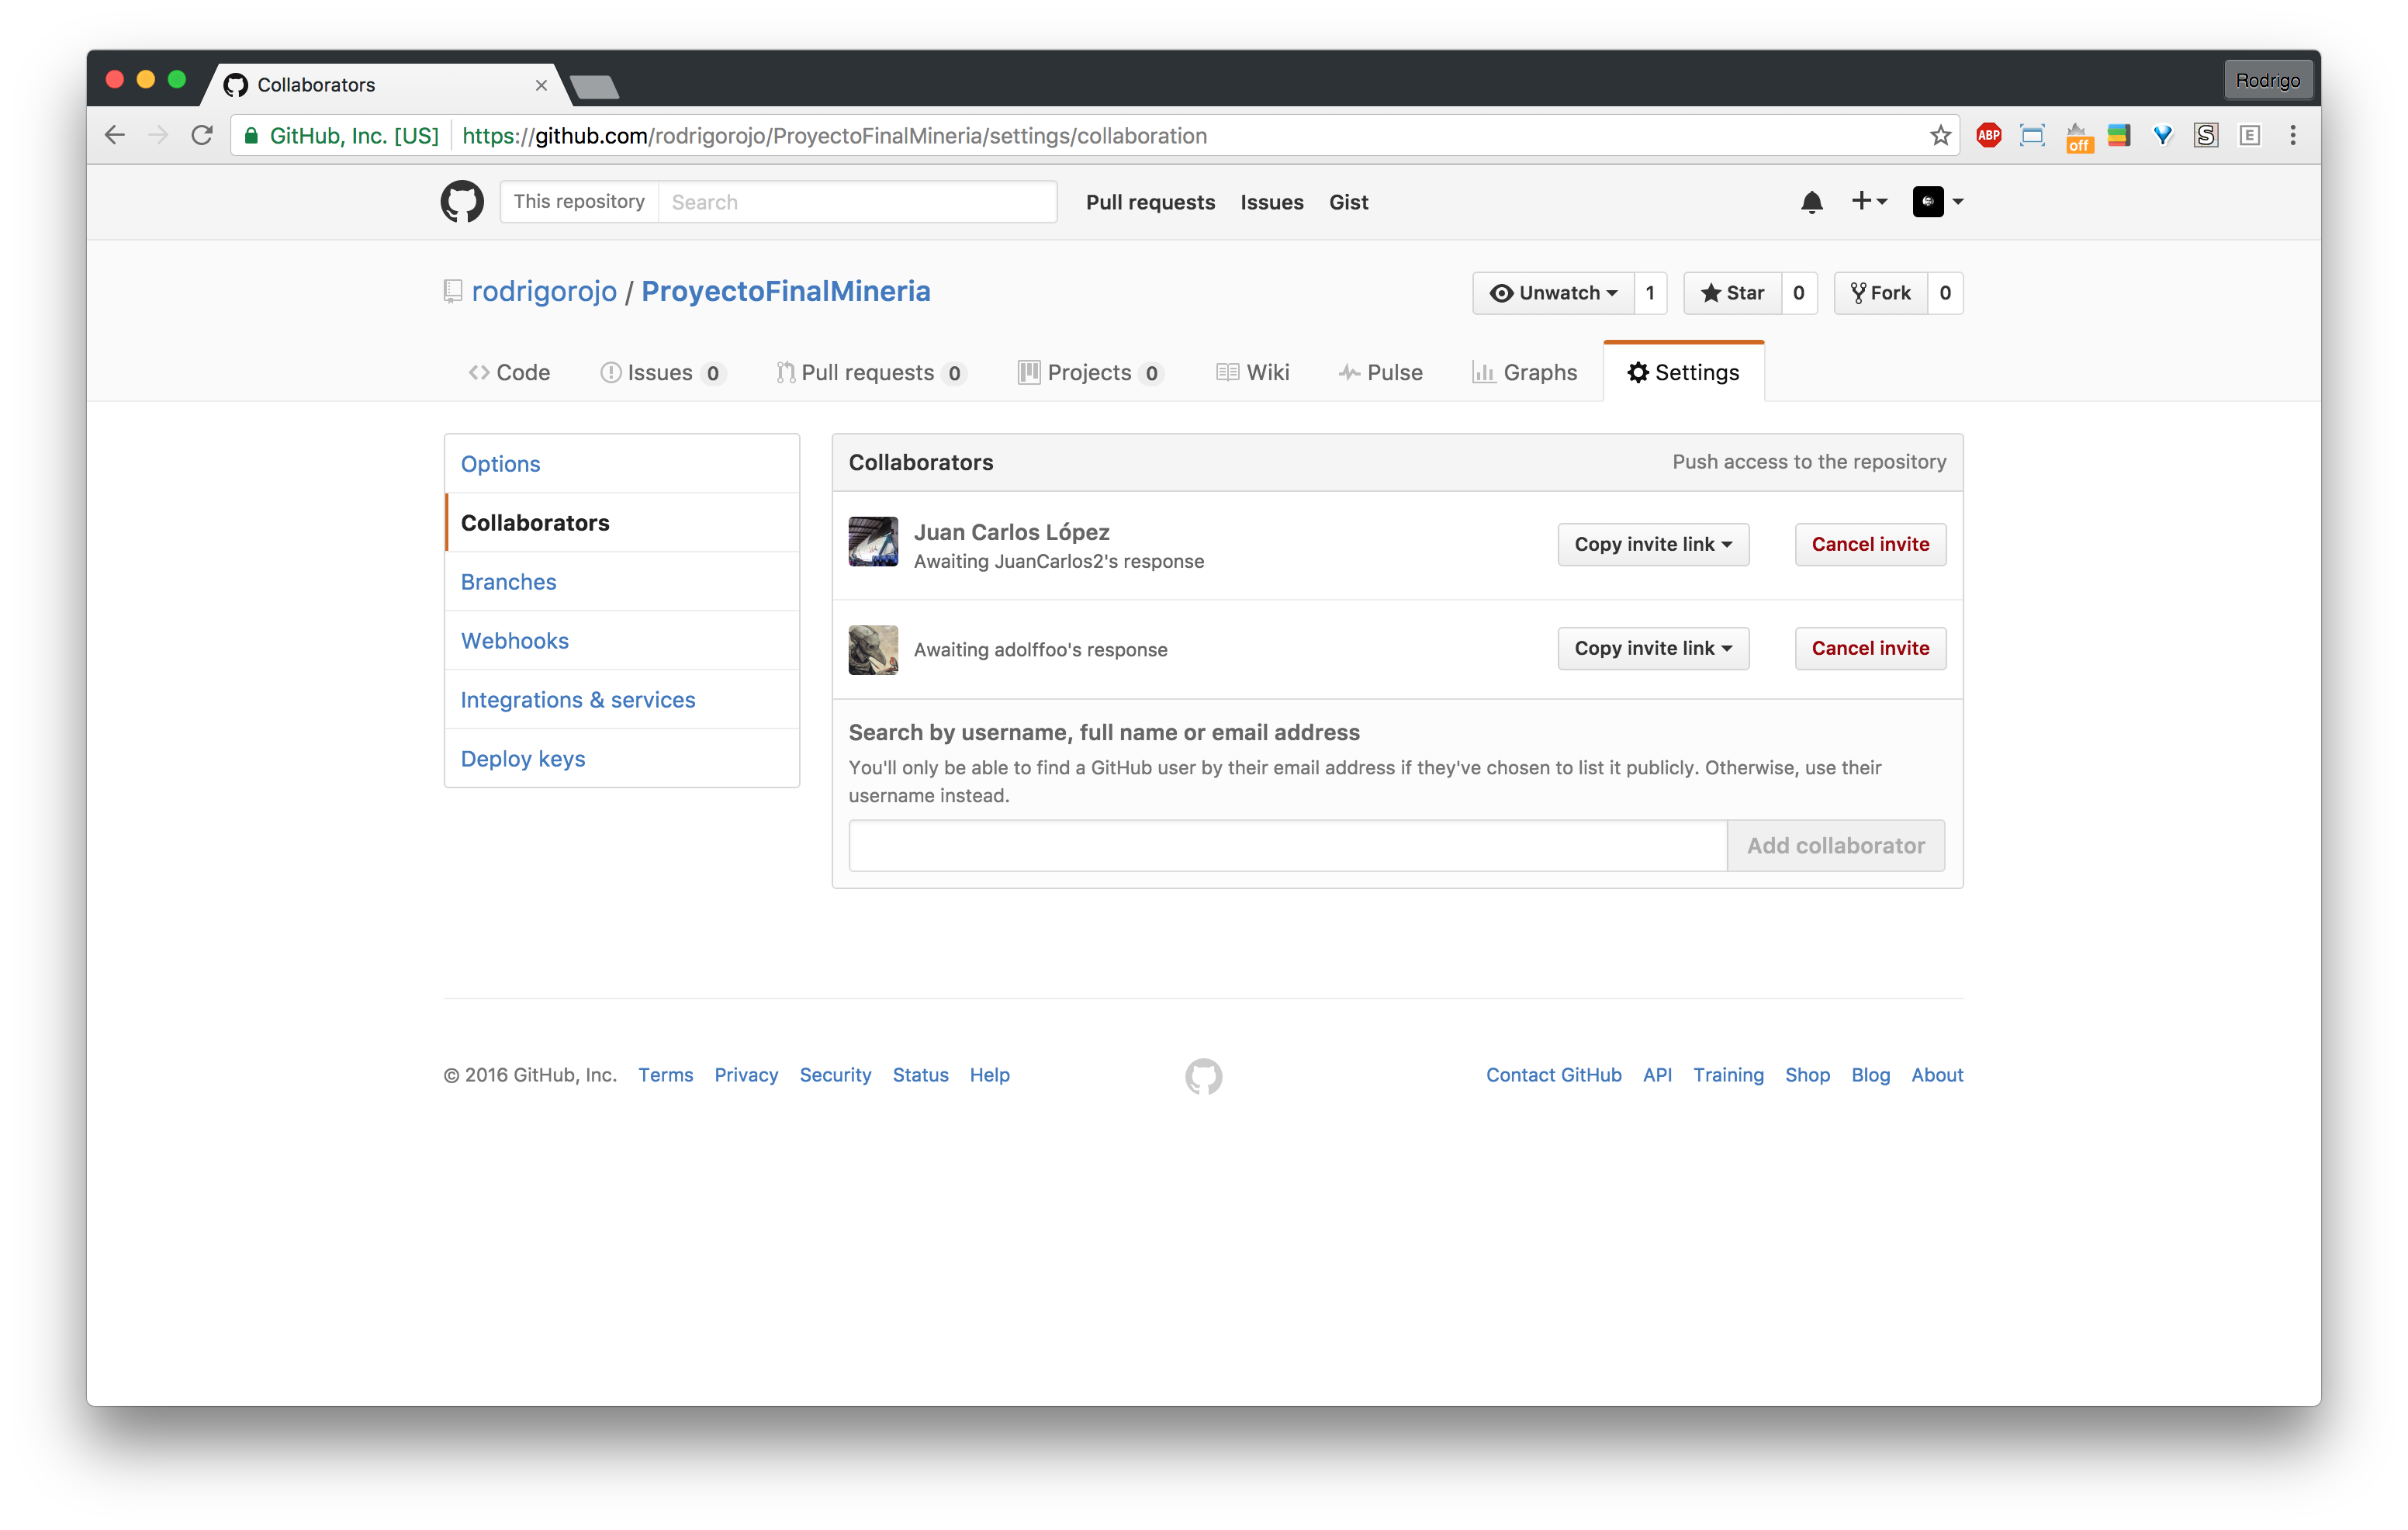
\includegraphics[scale=0.1]{7}
     \end{center}
     \textbf{Nota: Los primeros dos pasos ya fueron realizados, el repositorio se encuentra en: }\\
     https://github.com/rodrigorojo/ProyectoFinalMineria
     \item Clonar el repositorio: Esto lo haremos mediante SSH\\
     Abrimos una terminal en la carpeta en donde lo queremos clonar y ponemos:
     \begin{verbatim}
       $ git clone git@github.com:rodrigorojo/ProyectoFinalMineria.git
     \end{verbatim}
     \item Para actualizar el repositorio: nos ubicamos en la carpeta donde se encuentra, abrimos una terminal y ponemos:
     \begin{verbatim}
       $ git pull
     \end{verbatim}
     Se recomienda antes de empezar a trabajar en el repositorio hacer siempre este paso.
     \item Cada que realicemos cambios en el proyecto los debemos de agregar, hacer commit y subir. Esto se puede realizar de la siguiente manera:
     \begin{verbatim}
       $ git add .
       $ git commit -m "Nombre del commit"
       $ git push
     \end{verbatim}


   \end{enumerate}
 \end{itemize}
\end{document}
